\documentclass[twoside,11pt]{article}

% Any additional packages needed should be included after jmlr2e.
% Note that jmlr2e.sty includes epsfig, amssymb, natbib and graphicx,
% and defines many common macros, such as 'proof' and 'example'.
%
% It also sets the bibliographystyle to plainnat; for more information on
% natbib citation styles, see the natbib documentation, a copy of which
% is archived at http://www.jmlr.org/format/natbib.pdf

\usepackage{jmlr2e}
\usepackage{minted}
\usepackage[utf8]{inputenc} % allow utf-8 input
\usepackage{graphicx}
\usepackage{svg}
\usepackage{caption}
\usepackage{subcaption}
\usepackage{stmaryrd}
\usepackage[colorinlistoftodos]{todonotes}
\newcommand{\aurelien}[1]{\todo[inline,caption={},color=orange!40]{{\it Aurelien:~}#1}}
\newcommand{\william}[1]{\todo[inline,caption={},color=blue!40]{{\it William:~}#1}}
%\renewcommand{\aurelien}[1]{}


\graphicspath{{images/}}

% Definitions of handy macros can go here

\newcommand{\dataset}{{\cal D}}
\newcommand{\fracpartial}[2]{\frac{\partial #1}{\partial  #2}}

% Heading arguments are {volume}{year}{pages}{submitted}{published}{author-full-names}

\jmlrheading{}{}{}{}{}{William de Vazelhes and CJ Carey and Yuan Tang and Nathalie Vauquier and Aur\'elien Bellet}

% Short headings should be running head and authors last names

\ShortHeadings{metric-learn: Metric Learning Algorithms in Python}{de Vazelhes, Carey, Tang, Vauquier and Bellet}
\firstpageno{1}

\begin{document}

\title{metric-learn: Metric Learning Algorithms in Python}

\author{\name William de Vazelhes \email william.de-vazelhes@inria.fr \\
       \addr INRIA, France
       \AND
       \name CJ Carey \email perimosocordiae@gmail.com \\
       \addr \aurelien{CJ must put in his affiliation}
       \AND
       \name Yuan Tang \email terrytangyuan@gmail.com \\
       \addr Ant Financial, United States
       \AND
       \name Nathalie Vauquier \email nathalie.vauquier@inria.fr \\
       \addr INRIA, France
       \AND
       \name Aur\'elien Bellet \email aurelien.bellet@inria.fr \\
       \addr INRIA, France
       }

\editor{}

\maketitle

\begin{abstract}%   <- trailing '%' for backward compatibility of .sty file
\texttt{metric-learn} is an open source Python package implementing supervised and weakly-supervised distance metric learning algorithms. As part of \texttt{scikit-learn-contrib}, it provides a unified interface compatible with \texttt{scikit-learn} which allows to easily perform cross-validation, model selection, and pipelining with other machine learning estimators. \texttt{metric-learn} is thoroughly tested and available on PyPi under the MIT licence.
%The source code is available online at \url{http://github.com/scikit-learn-contrib/metric-learn}, as well as the documentation at \url{http://metric-learn.github.io/metric-learn/}.
\end{abstract}

\begin{keywords}
  Machine Learning, Python, Metric Learning, Scikit-learn
\end{keywords}

\section{Introduction}

Many approaches in machine learning require a measure of distance between data
points. Traditionally, practitioners would choose a standard distance metric
(Euclidean, City-Block, Cosine, etc.) using a priori knowledge of the
domain. However, it is often difficult to design metrics that are well-suited
to the particular data and task of interest.
% \todo[inline]{probably need to add a sentence explaining what is meant by weak supervision}
Distance metric learning, or simply metric learning \citep{Bellet15,Kulis13}, aims at
automatically constructing task-specific distance metrics from data, in a machine learning manner. A key advantage of metric learning is that it can be applied beyond the standard supervised learning setting (data points associated with labels), in situations where only weaker forms of supervision are available (e.g., pairs of points that should be similar/dissimilar). The learned distance metric can
then be used to perform various tasks, for instance to retrieve the elements (images, documents) of a database that are semantically closer to a query element. It can also be plugged into other machine learning algorithms: popular use-cases include improving the accuracy of nearest neighbors learning models (for classification, regression, anomaly detection...) or biasing the clusters found by clustering algorithms like K-Means towards the intended semantics. Finally, metric learning can be used to perform dimensionality reduction.
These use-cases highlight the importance of integrating metric learning into the rest of the machine learning pipeline and tools.
% \todo[inline]{quick presentation of the package: implements several algorithms, with sklearn-compatible API for model selection, model evaluation, pipelining with other estimators. makes metric-learn stands out from other packages (maybe mention a few of them), in particular in the case of weakly supervised algorithms}

\texttt{metric-learn} is an open source package for metric learning in Python, which implements many popular metric-learning algorithms with different levels of supervision through a unified interface.
%\footnote{This makes \texttt{metric-learn} stand out from other packages, like \texttt{PyDML} (\url{https://github.com/jlsuarezdiaz/pyDML}) which focuses on supervised metric learning algorithms.}
% (not only class supervision, unlike most packages are focused on, including another package for metric learning in Python, \texttt{PyDML})
% , which is one interesting feature allowed by the metric learning paradigm. 
Its API is compatible with scikit-learn, the leading library for machine learning in Python, allowing for streamlined model selection, evaluation, and pipelining with other estimators.
The project is developed collaboratively through GitHub, its code is thoroughly tested using continuous integration tools. It was recently included to \texttt{scikit-learn-contrib}, which hosts high-quality \texttt{scikit-learn}-compatible projects.\footnote{\url{https://github.com/scikit-learn-contrib/scikit-learn-contrib}}
\aurelien{decide if we include or not a few sentences on positioning wrt other packages}

%, which makes \texttt{metric-learn} stand out from other packages, like \texttt{PyDML} \footnote{\url{https://github.com/jlsuarezdiaz/pyDML}}, which mostly focuses on supervised metric learning algorithms.
% Acknowledgements should go at the end, before appendices and references
%The rest of this paper is organized as follows. We first present an overview of the package, followed by a more detailed description of the available algorithms. We then give more details about the API and the software architecture, in particular the compatibility with \texttt{scikit-learn}, and conclude with a discussion of future developments.

% \aurelien{we could put the presentation of metric learning and supervision as Sec 2, and put the implemented algorithms in the overview of the package section as Section 3}

\section{Background on Metric Learning} \label{metriclearning}

% \todo[inline]{comparison with other packages ? }
% Metric learning problems fall into two main categories depending on the type
% of supervision available about the training data:

% \begin{itemize}
%     \item 
% - Supervised learning: the algorithm has access to
%   a set of data points, each of them belonging to a class (label) as in a
%   standard classification problem.
%   Broadly speaking, the goal in this setting is to learn a distance metric
%   that puts points with the same label close together while pushing away
%   points with different labels.
% - Weakly supervised learning: the
%   algorithm has access to a set of data points with supervision only
%   at the tuple level (typically pairs, triplets, or quadruplets of
%   data points). A classic example of such weaker supervision is a set of
%   positive and negative pairs: in this case, the goal is to learn a distance
%   metric that puts positive pairs close together and negative pairs far away.


% \end{itemize}


% \paragraph{General setting} Metric learning problems are generally formulated as an optimization problem where one seeks to find, on the training data $(x_0, ..., x_n)$, the parameters $\theta$ of a distance function $D_\theta(x_i, x_j)$ that optimize some desired objective function $\mathcal{L}_\theta(x_0, ..., x_n) = f(D_\theta(x_0, x_0), ..., D_\theta(x_0, x_n), ..., D_\theta(x_n, x_0), ..., D_\theta(x_n, x_n))$, hoping that this metric will generalize the desired propertie(s) on new incoming test data.

Metric learning is generally formulated as an optimization problem where one seeks to find the parameters of a distance function that minimize some objective function over the input data.
All algorithms currently implemented in \texttt{metric-learn} learn so-called Mahalanobis distances. Given a real-valued parameter matrix $L$ of shape \texttt{(n\_components, n\_features)} where \texttt{n\_features} is the
number of features describing the data, the associated Mahalanobis distance between two points $x$ and $x'$ is defined as $D_L(x, x') = \sqrt{(Lx-Lx')^\top(Lx-Lx')}$.
This is equivalent to a Euclidean distance after the linear transformation of the feature space defined by $L$ (taking $L$ to be the identity matrix recovers the standard Euclidean distance).
Mahalanobis distance metric learning can thus be seen as learning a new
embedding space of (potentially reduced) dimension \texttt{n\_components}.
Note that $D_L$ can also be written as $D_L(x, x') = \sqrt{(x - x')^\top M (x - x')}$, where $M = L^\top L$ is called the Mahalanobis matrix.

% Strictly speaking, Mahalanobis distances are "pseudo-metrics": they satisfy
% three of the properties of a metric (non-negativity, symmetry, triangle inequality) but not
% necessarily the identity of indiscernibles.

% Mahalanobis distances can also be parameterized by a positive semi-definite 
% (PSD) matrix $M$:

% $ D(x, x') = \sqrt{(x-x')^\top M(x-x')}$

% Using the fact that a PSD matrix :math:`M` can always be decomposed as
% $M=L^\top L$ for some  :math:`L`, one can show that both
% parameterizations are equivalent. In practice, an algorithm may thus solve
% the metric learning problem with respect to either :math:`M` or :math:`L`.

Metric learning algorithms can be classified according to the form of data supervision that they need to learn the metric. \texttt{metric-learn} currently implements algorithms that fall into the following categories:
\begin{itemize}
\item \textbf{Supervised learners} learn from a standard labeled dataset and essentially aim to bring closer together points from the same class while spreading further away points from a different class. For instance, the class may be the identity of a person in an image (see Figure~\ref{fig:full}). 
% \todo[inline]{ces figures ne sont pas très vendeuses. je propose de faire une figure conceptuelle en prenant l'exemple des faces expliquant la différence entre le supervisé, les paires et les quadruplets. on peut s'inspirer de \url{http://cedric.cnam.fr/~thomen/papers/Law_ICCV_2013_QWise.pdf}}
% \begin{figure}[H]
% \centering
% \begin{subfigure}{.5\textwidth}
%   \centering
%   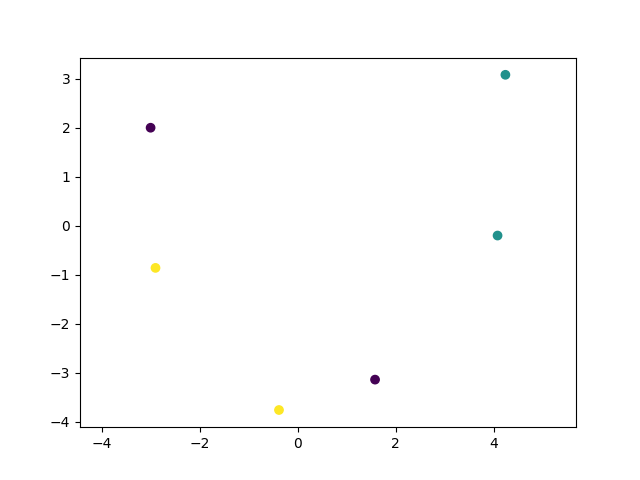
\includegraphics[width=.8\linewidth]{supervised_without_metric.png}
%   \caption{Original points, before metric learning}
%   \label{fig:sub1}
% \end{subfigure}%
% \begin{subfigure}{.5\textwidth}
%   \centering
%   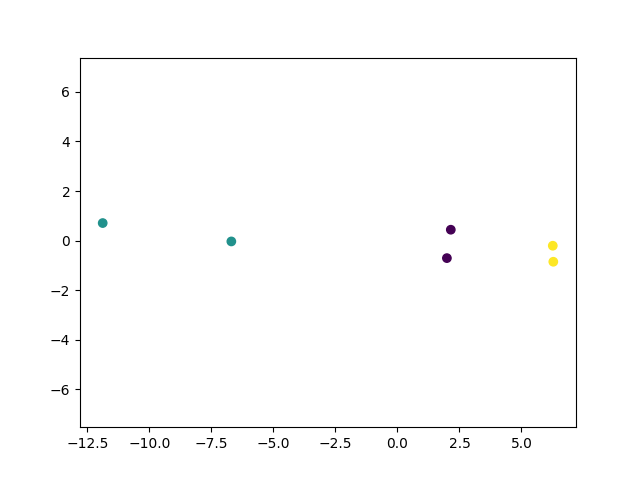
\includegraphics[width=.8\linewidth]{supervised_with_metric.png}
%   \caption{points after metric learning (ITML)}
%   \label{fig:sub2}
% \end{subfigure}
% \caption{Metric learning with pairwise constraints}
% \label{fig:test}
% \end{figure}
% \paragraph{Weakly Supervised Metric Learning algorithms}
% Weakly Supervised algorithms use less information than the previous algorithms: they only take tuple of points and possibly a corresponding label. See below for more concrete examples of algorithms learning on tuples.
\item \textbf{Pair learners} take as input a set of pairs of points with a pair label indicating whether the two points are similar or not. They aim to learn a metric that brings points from a similar pair closer together, and points from a dissimilar pair further away from each other. Such weak supervision is often simpler to collect than class labels in applications when there are many labels. %, since annotators will only need to say whether images are similar or not, and will not have to assign a label in a huge list of those.
For instance, an annotator can easily decide whether two face images correspond to the same person while it can be difficult to match a face to its identity among a large number of people (see Figure~\ref{fig:pairs}). 
% \begin{figure}[H]
% \centering
% \begin{subfigure}{.5\textwidth}
%   \centering
%   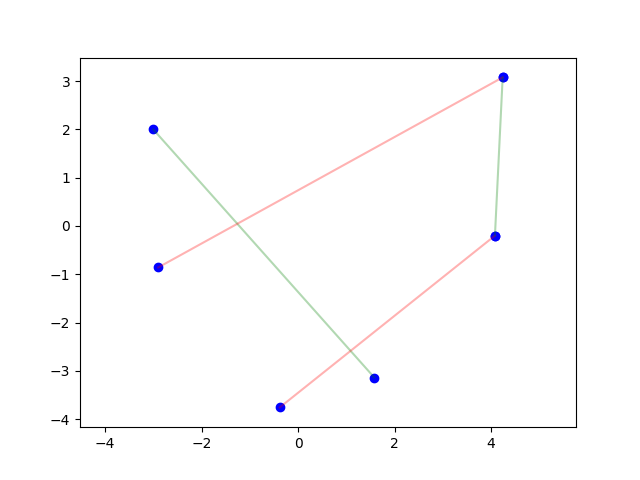
\includegraphics[width=.8\linewidth]{pairs_without_metric.png}
%   \caption{Original points, before metric learning}
%   \label{fig:sub1}
% \end{subfigure}%
% \begin{subfigure}{.5\textwidth}
%   \centering
%   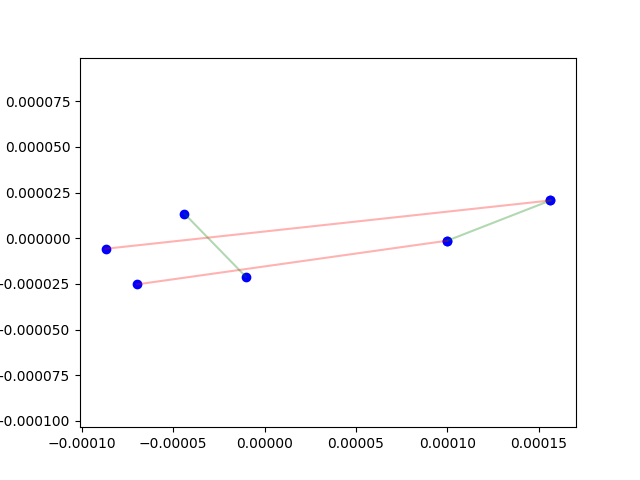
\includegraphics[width=.8\linewidth]{pairs_with_metric.png}
%   \caption{points after metric learning (ITML)}
%   \label{fig:sub2}
% \end{subfigure}
% \caption{Metric learning with pairwise constraints}
% \label{fig:test}
% \end{figure}
\item \textbf{Quadruplet Learners} take as input quadruplets of points and aim to learn a metric that brings the two first points of each quadruplet closer than the two last points. This can be useful to learn a metric space in which closer points have closer values of an attribute that is not binary like in pair supervision (e.g. same person/not same person) but rather continuous and difficult to annotate precisely (e.g., the age of a person on an image, see Figure \ref{fig:quadruplets}).
%for instance, we want to learn a metric that puts closer together people from approximately the same age.
\end{itemize}




\begin{figure}[t]
  \begin{subfigure}
     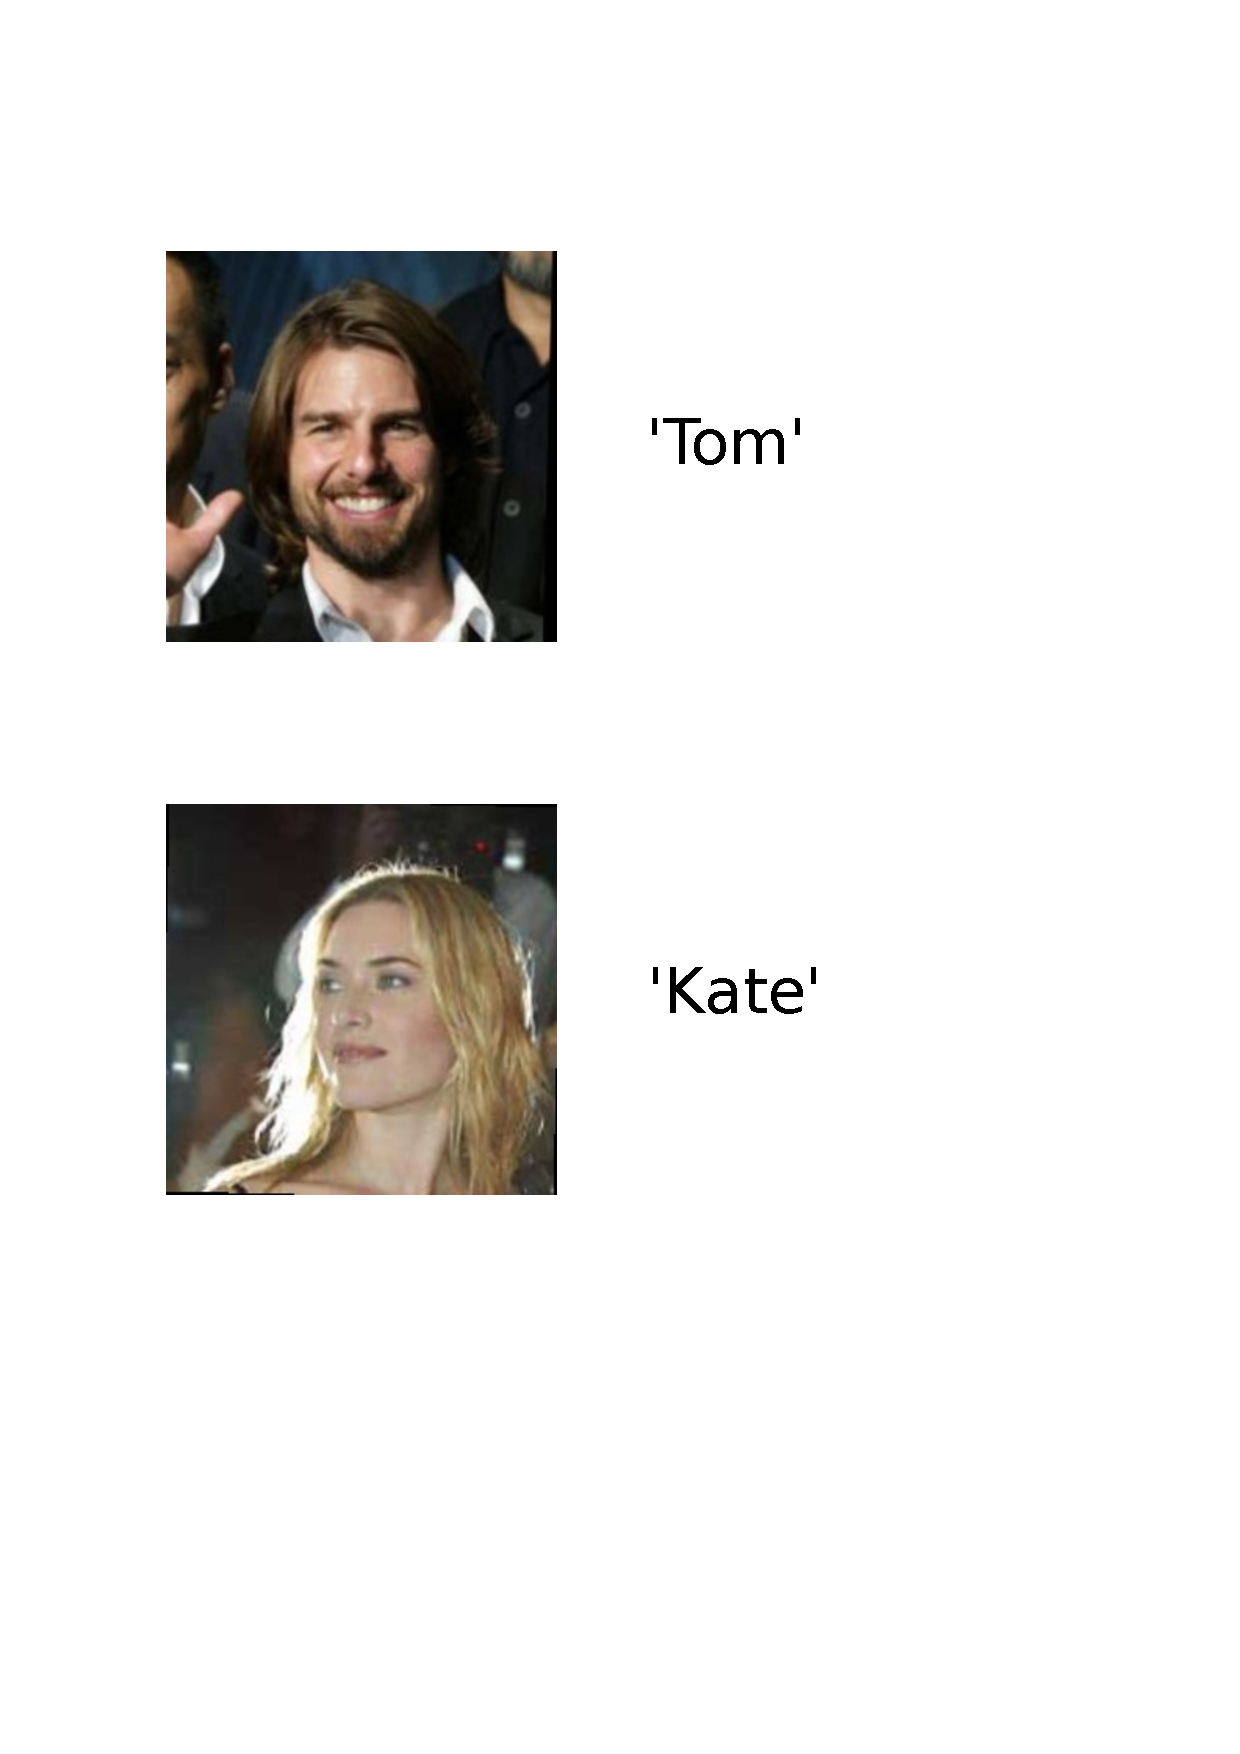
\includegraphics[scale=0.2]{labels.pdf}
     \label{fig:full}
\end{subfigure}
 \begin{subfigure}
     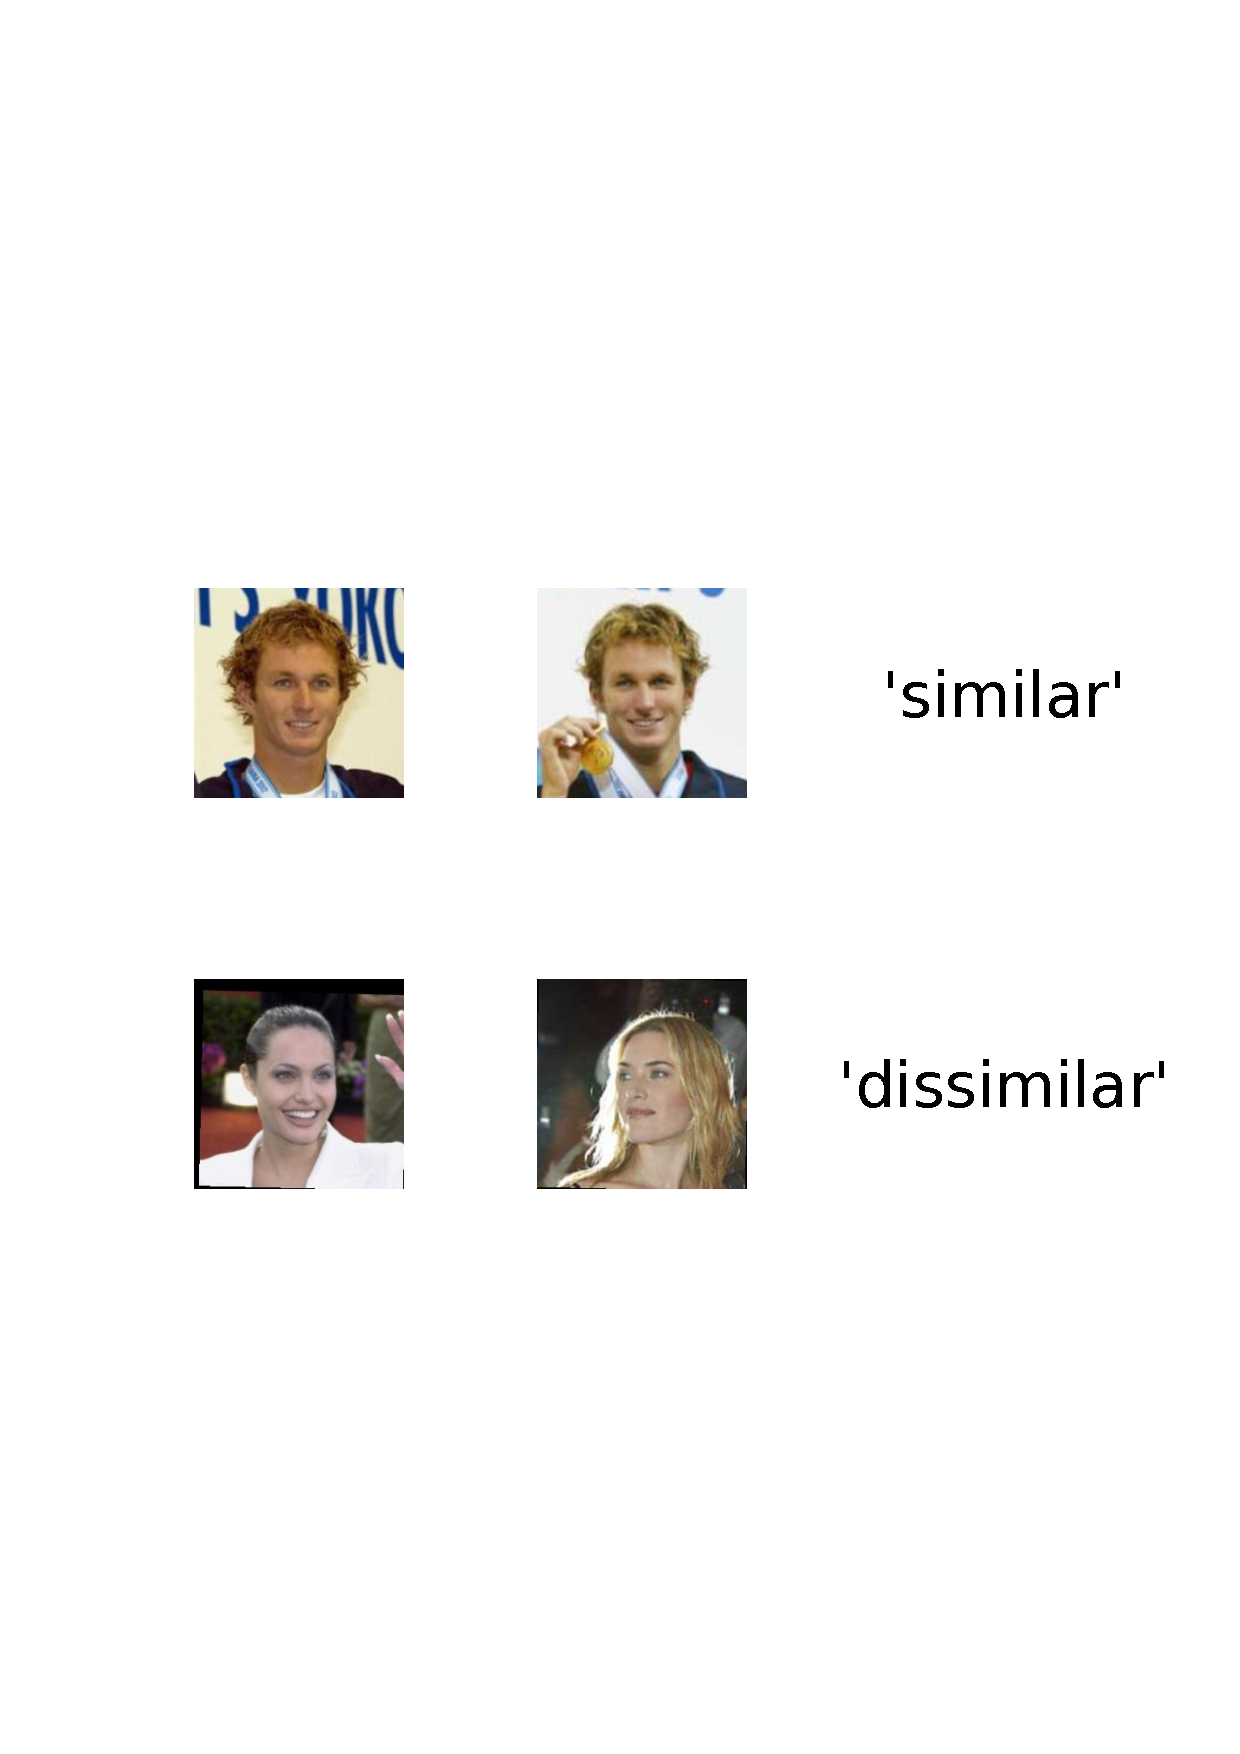
\includegraphics[scale=0.2]{pairs.pdf}
     \label{fig:pairs}
  \end{subfigure}
\begin{subfigure}
     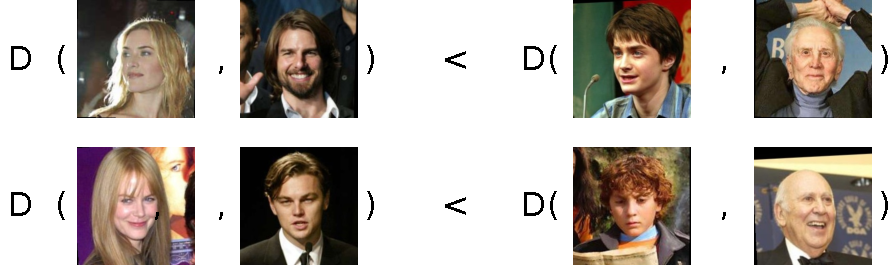
\includegraphics[scale=0.2]{quadruplets.pdf}
     \label{fig:quadruplets}
  \end{subfigure}
  \caption{Different types of supervision for metric learning. (\subref{fig:full}) Full supervision: make samples from the same label (here, identity) closer together than samples from different labels. (\subref{fig:pairs}) Pair supervision: make similar pairs (here, corresponding to the same person) to be closer than dissimilar pairs (different persons). (\subref{fig:quadruplets}) Quadruplet supervision: make the two leftmost samples (here, people of similar age) to be closer than the two rightmost samples (of bigger age difference). Images are taken from the Labeled Faces in the Wild dataset \citep{Huang12}.}
  \label{fig:contour}
\end{figure}



\section{Overview of the Package}

The current release of \texttt{metric-learn} (v.0.5.0) can be installed from the Python Package Index (PyPI), for python 2.7 and 3.5 or later. The source code is available on GitHub at \url{http://github.com/scikit-learn-contrib/metric-learn} and is free of use, provided under the MIT licence. A detailed documentation (including installation guidelines, the description of the algorithms and the API, as well as examples) is available at \url{http://contrib.scikit-learn.org/metric-learn}.


\texttt{metric-learn} only relies on core libraries from the SciPy ecosystem: \texttt{numpy}, \texttt{scipy}, and \texttt{scikit-learn}. The development is collaborative and open to all contributors through the usual GitHub framework (issues and pull requests). The interest of the package from the community is clear: it has been included in \texttt{scikit-learn-contrib} and, at the time of writing, has been starred more than 740 times and forked more than 170 times.
The quality of the code is ensured by a thorough test coverage (96\% as of July 2019). Every new contribution to the code is automatically checked by a continuous integration platform that ensures a minimal test coverage of the added code, a minimal variation in test coverage of the overall project, and syntax formatting with \texttt{flake8}. %, which allows easy contribution for incoming developers, which can have their code automatically checked.

Currently, \texttt{metric-learn} implements 9 popular metric learning algorithms from the literature. Supervised learners include Neighborhood Components Analysis \citep[NCA,][]{Goldberger04}, Large Margin Nearest Neighbors \citep[LMNN,][]{Weinberger09}, Relative Components Analysis \citep[RCA,][]{Shental02},\footnote{Strictly speaking, RCA takes as input slightly weaker supervision in the form of \emph{chunklets} (groups of points from the same class).} Local Fisher Discriminant Analysis \citep[LFDA,][]{Sugiyama07} and Metric Learning for Kernel Regression \citep[MLKR,][]{Weinberger07}. Note that the latter is designed for regression problems and takes as input continuous labels. Pair learners include Mahalanobis Metric for Clustering (MMC) (\cite{Xing2002a}), Information Theoretic Metric Learning (ITML) (\cite{Davis07}) and Sparse High-Dimensional Metric Learning (SDML) (\cite{Qi09}). Finally, the package implements one quadruplet learner: Metric Learning from Relative Comparisons by Minimizing Squared Residual (LSML) (\cite{Liu12}). Detailed descriptions of these algorithms can be found in the package documentation.

\section{Software Architecture and API}

\aurelien{mention optimization somewhere?}
\texttt{metric-learn} provides a unified interface to all metric learning algorithms (including the weakly supervised ones that have an input format that differs from the classic machine learning settings) and is designed to be fully compatible with the functionalities of \texttt{scikit-learn} \citep{scikit-learn}. All metric learners in \texttt{metric-learn} inherit from an abstract \texttt{BaseMetricLearner} object, which itself inherits from scikit-learn's \texttt{BaseEstimator}. All classes inheriting from \texttt{BaseMetricLearner} should implement two methods, \texttt{get\_metric} and \texttt{score\_pairs}: the former returns a function that computes the distance between two points $u$ and $v$. The latter method computes the distances between a dataset of pairs of points.
\aurelien{score\_pairs and get\_metric should be mentioned here (all metric learners should implement these). In Mahalanobis, just mention they are implemented accordingly (do not delete: TODO: update accordingly mahalanobis}
% \todo[inline]{Should I talk about the classes etc ? Not useful since they are not visible by the user right ?}
% \todo[inline]{I think it can be nice, this is not documentation, but explaining how things are coded}

%\texttt{metric-learn}'s API is designed to be fully compatible with \texttt{scikit-learn} API (\cite{scikit-learn}). 

\paragraph{Mahalanobis metric learning}

Since they learn a Mahalanobis matrix, all algorithm also inherit from the \texttt{MahalanobisMixin} interface. This latter can return the mahalanobis matrix with the method \texttt{get\_mahalanobis\_matrix}. Like scikit-learn's algorithms, it can also return a \texttt{components\_} attributes that is the transformation matrix \texttt{L}. Since all these metric learner learn this implicit transformation $L$, they can project the input in the new space using \texttt{transform}. A distance function can also be extracted from them using \texttt{get\_metric}, that can further be used in any scikit-learn estimator like \texttt{KMeansClustering}. They can also return the distance between a dataset of pairs (in the 3D array format (see below), using \texttt{score\_pairs}.



\paragraph{Supervised metric learners}


Supervised metric learners inherit from scikit-learn base class \texttt{TransformerMixin}, just like \texttt{scikit-learn}'s \texttt{LinearDiscriminantAnalysis} for instance. As such, they are compatible with pipelining (\texttt{sklearn.pipeline.Pipeline} and \texttt{sklearn.pipeline.make\_pipeline}.
% (they pass all scikit-learn's "estimators checks"). 
%  They can easily be pipelined with nearest neighbors estimators to improve their performance: \texttt{better\_knn = sklearn.pipeline.make\_pipeline(NCA(), KNeighborsClassifier())} (TODO: sth to explain NCA is in metric-learn)
\aurelien{mention pipelining}

\william{cf. Nathalie's comment: re-introduce weakly supervised metric laerners}
\paragraph{Weakly Supervised metric learners} 
% Algorithms that learn on pairs or quadruplets take as input 3D array of shape \texttt{(n\_samples, t, n\_features)} (where...). In other words, sampling one element along the first dimension returns one tuple (e.g. a pair), that is a matrix of t lines corresponding to the t elements in the tuple.
% This format is what allows all these API choices, since slicing along the 1st dimension
% While a classical input array \texttt{X} in \texttt{scikit-learn} has shape \texttt{(n\_samples, n\_features)}, an array of tuples has shape \texttt{(n\_tuples, t, n\_features)}, where \texttt{t} is the number of elements in a tuple (e.g. 2 for pairs).
% Note that \texttt{scikit-learn} accepts arrays in a broad sense, in what they call "array-like" objects. \texttt{metric-learn} too accepts "tuple-like" objects.
Weakly supervised learning algorithms are similar to \texttt{scikit-learn} classifiers, but they \texttt{fit} on tuples that can be given as 3D arrays, instead of 2D arrays-like of points \texttt{X}. They have a \texttt{predict} method, that gives a prediction for each given tuple (e.g. for pairs it predicts whether the two points in a pair or similar or not). Tuples can be pairs or quadruplets, depending on the specific algorithm used. (see section~\ref{metriclearning}). Say we work with $n_t$ tuples of points with $p$ features each.\\
\textit{(i) Pairs learners} take as input an array-like \texttt{pairs} of shape $(n_t, 2, p)$, as well as an array-like \texttt{y\_pairs} of shape $(n_t,)$, which for each pair tells whether it contains similar or dissimilar samples. In order to \texttt{predict} on incoming pairs whether they are similar or not, they also need to fit a threshold, i.e. a reference distance with respect to which the distance between the incoming points will be compared. If this distance is higher than the threshold, the pair will be predicted as dissimilar, and if smaller as similar. This threshold is automatically fitted at fit time using a heuristic, but can be set manually using the method \texttt{set\_threshold}, or calibrated more specifically on a validation set, in order to optimize any classification score, using the method \texttt{calibrate\_threshold}.\\
\textit{(ii) Quadruplets learners} work on arrays-like of shape $(n_t, 4, p)$, and no labels array, where for each quadruplet the two first elements are the ones we want to be closer than the two last ones. They can also \texttt{predict} whether an incoming quadruplet is in the right order or not, i.e. whether the two first elements are indeed more similar that the two last, by comparing the two pairwise distances.
\aurelien{a bit more details would be welcome (explain both case of pairs and quadruplets). for pairs, need to mention threshold and calibration.}

\begin{minted}[%linenos=TRUE,
fontsize=\footnotesize]{python}
>>> from sklearn.model_selection import train_test_split, cross_val_score
>>> from sklearn.datasets import fetch_lfw_pairs
>>> from metric_learn import ITML  
>>> dataset = fetch_lfw_pairs(resize=0.2)  
>>> pairs, y_pairs = ((dataset.pairs.reshape(2200, 2, -1) - 127.5) / 255, 
                      2 * dataset.target - 1)
>>> pairs, _, y_pairs, _ = train_test_split(pairs, y_pairs, train_size=1000, 
                                            stratify=y_pairs, random_state=42) 
>>> itml = ITML(prior='random', random_state=42)  
>>> cross_val_score(itml, pairs, y_pairs, scoring='accuracy')
array([0.62275449, 0.65165165, 0.63963964])
\end{minted}
% mmc.predict(pairs)

\aurelien{the snippet does not work, cannot do 3-fold CV on 2 samples.. maybe we can load a subset of pairs from LFW? ideally we should also include the imports so the snippet is self-sufficient. to save space, maybe we can split this over 2 columns, with line numbering or something}
\william{new snippet takes large horizontal space, still split ?}
This allows to use out of the box \texttt{scikit-learn}'s scoring functions, and therefore all routines for model selection, including the \texttt{GridSearchCV} object. Also note that for every weakly supervised learner, there is a \texttt{\_Supervised} version (e.g. for \texttt{MMC} there is \texttt{MMC\_Supervised}, that is a supervised version that samples pairs of similar samples from intra-class samples, and dissimilar samples from inter-class samples, and fits \texttt{MMC} on these pairs).


% \begin{minted}{python}
% from sklearn.model_selection import GridSearchCV
% model = GridSearchCV(mmc, {'init': ['random', 'identity', 'covariance']})
% model.fit(pairs, y_pairs)
% \end{minted}

\section{Conclusion and Future Work}

\texttt{metric-learn} is under active development --- we list here some promising directions to further improve the package. Regarding scalability to large datasets, we would like to implement stochastic solvers (stochastic gradient descent and its variants), forming batches of tuples on the fly to avoid loading all data in memory at once. We would also like to offer better support to inputs in sparse format.
Finally, we are looking to incorporate additional algorithms that provide added value to the package, in particular triplet metric learners and algorithms that can deal with multi-label problems \citep{liu15} and high-dimensional data \citep{Liu19}.
%We could also allow metric learn to be used when having multiple labels for each sample, and allow different kind of supervisions, like semi-supervised learning for instance.
%We could also improve the ease of use by adding more examples and adding toy datasets to play with quickly and see the interest of the weaker forms of supervision. About the overall quality of the software, we intend to improve the continuous integration routines, for instance by ensuring a PEP8 syntax checker is run on every pull request, a continuous integration for the documentation.

\acks

We are particularly thankful to Inria for funding two years of development of the package. We also thank \texttt{scikit-learn} developers from the Inria Parietal team (in particular Gaël Varoquaux, Alexandre Gramfort and Olivier Grisel) for fruitful discussions on the design of the API and for providing some conference funding, as well as scikit-learn-contrib reviewers who integrated the package in the organisation. 
\aurelien{potentially mention contrib reviewers if we are accepted.: include rth and adrinjalali ?}


%  The quality of comparison to previous (if any) related implementations, w.r.t. run-time, memory requirements, features, to explain that significant progress has been made. 

% Manual newpage inserted to improve layout of sample file - not
% needed in general before appendices/bibliography.

\bibliography{metric-learn-jmlr}

\end{document}